% Section content template for individual Educative lessons
% This file contains the actual content for a specific section
% Generated from Educative API section content

% Section: Design of a Distributed Messaging Queue: Part 1
% Section ID: 6330012742975488
% Section Slug: design-of-a-distributed-messaging-queue-part-1
% Generated: 2025-12-07T20:58:12.277000

So far, we've discussed the requirements and design considerations of a distributed messaging queue. Now , let's begin with learning about the high-level design of a distributed messaging queue.

\subsection{Distributed messaging queue}\label{cVs9CHmu_02fDJDr3TrXK}
\\
Unlike a single-server messaging queue, a distributed messaging queue resides on multiple servers. A distributed messaging queue has its own challenges. However, it resolves the drawbacks of a single-server messaging queue if designed properly.\\
\strut \\
The following sections focus on the scalability, availability, and durability issues of designing a distributed messaging queue by introducing us to a more fault-tolerant architecture of a messaging queue.\\

\subsubsection{High-level design}\label{BUL_3j01HlttPPyStyVfT}
\\
Before diving deep into the design, let's assume the following points to make the discussion more simple and easy to understand. In the upcoming material, we discuss how the following assumptions enable us to eliminate the problems in a single-server solution to the messaging queue.

\begin{enumerate}
\item
\protect\phantomsection\label{3O_8xehomqbPVTRAM1-mT}
Queue data is replicated using either a primary-secondary or quorum-like system inside a cluster (read through the \href{https://www.educative.io/courses/grokking-the-system-design-interview/data-replication}{Data Replication} lesson for more details). Our service can use data partitioning if the queue gets too long to fit on a server. We can use a consistent hashing-like scheme for this purpose, or we may use a key-value store where the key might be the sequence numbers of the messages. In that case, each shard is appropriately replicated (refer to the \href{https://www.educative.io/courses/grokking-the-system-design-interview/data-partitioning}{Partition} lesson for more details on this).
\item
\protect\phantomsection\label{9fOX1FiWAN0f8cVxO9Qu3}
We also assume that our system can auto-expand and auto-shrink the resources as per the need to optimally utilize resources.
\end{enumerate}
\\
The following figure demonstrates a high-level design of a distributed messaging queue that's composed of several components.

\begin{figure}[htbp]
 \centering
 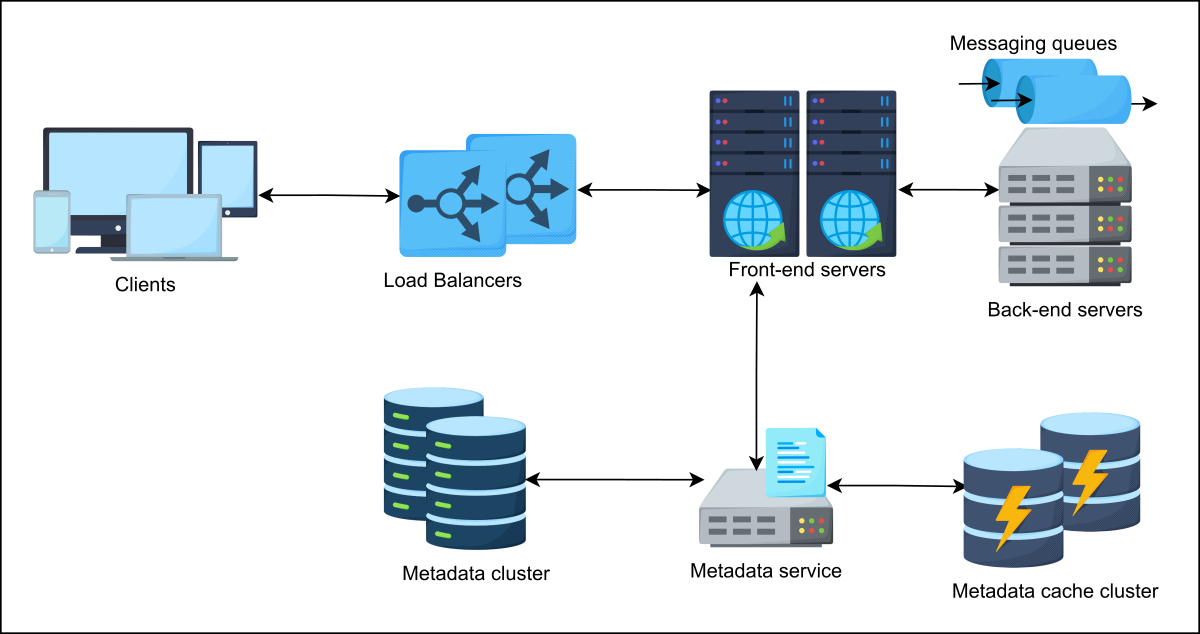
\includegraphics[width=0.5\textwidth]{Images/chapter_17/section_6330012742975488/6023326697127936.png}
 \caption{High-level architecture of distributed messaging queue}
\end{figure}

The essential components of our design are described in detail below.
\\
\paragraph{Load balancer}\label{RRVE_NREeYTSk2HeQBPTW}
\\
The load balancer layer receives requests from producers and consumers, which are forwarded to one of the front-end servers. This layer consists of numerous load balancers. Therefore, requests are accepted with minimal latency and offer high availability.
\\
\paragraph{Front-end service}\label{xbhKvihrHonqFJaGUh1uG}
\\
The front-end service comprises stateless machines distributed across data centers. The front-end provides the following services:

\begin{itemize}
\item
\protect\phantomsection\label{OWNXV9zV2_TXwdaFSQP5b}
\textbf{Request validation:} This ensures the validity of a request and checks if it contains all the necessary information.
\item
\protect\phantomsection\label{ae0lLGsCZRjB1O_ZdICz4}
\textbf{Authentication and authorization:} This service checks if the requester is a valid user and if these services are authorized for use to a requester.
\item
\protect\phantomsection\label{PPlWWSTjiF7SpxYt_JCga}
\textbf{Caching:} In the front-end cache, metadata(The metadata of a messaging queue typically includes essential information such as the queue's name, attributes, configuration settings, and may also encompass details like message retention policies, access permissions, and queue-specific metrics. It serves as a crucial reference for managing the behavior and characteristics of the messaging queue within a distributed system.) information is stored related to the frequently used queues. Along with this, user-related data is also cached here to reduce request time to authentication and authorization services.
\item
\protect\phantomsection\label{xYmTNWypilnf9Gb1_edwl}
\textbf{Request dispatching:} The front-end is also responsible for calling two other services, the back-end and the metadata store. Differentiating calls to both of these services is one of the responsibilities of the front-end.
\item
\protect\phantomsection\label{eZcs8UJ5B4_44OI_0_8j4}
\textbf{Request deduplication:} The front-end also tracks information related to all the requests, therefore, it also prevents identical requestsDeduplication from being put in a queue. Deciding what to do about duplicates might be as easy as searching a hash key in a store. If something is found in the store, this implies a duplicate and the message can be rejected.
\item
\protect\phantomsection\label{553-1lp9hz6VB6O3OW2vw}
\textbf{Usage data collection:} This refers to the collection of real-time data that can be used for audit purposes.
\end{itemize}
\\
\paragraph{Metadata service}\label{8E9O2PWYZL8_W94L4lHb_}
\\
This component is responsible for storing, retrieving, and updating the metadata of queues in the metadata store(A cluster of persistent data storage responsible for storing metadata related to all the queues available in the system.) and cache(A cluster of metadata, frequently accessed whenever clients' requests arrive.). Whenever a queue is created or deleted, the metadata store and cache are updated accordingly. The metadata service acts as a middleware between the front-end servers and the data layer. Since the metadata of the queues is kept in the cache, the cache is checked first by the front-end servers for any relevant information related to the receipt of the request. If a cache miss occurs, the information is retrieved from the metadata store and the cache is updated accordingly.
\\
There are two different approaches to organizing the metadata cache clusters:

\begin{enumerate}
\item
\protect\phantomsection\label{diEJr5YDK6ZFy35QldQIM}
If the metadata that needs to be stored is small and can reside on a single machine, then it's replicated on each cluster server. Subsequently , the request can be served from any random server. In this approach, a load balancer can also be introduced between the front-end servers and metadata services.
\end{enumerate}

\begin{figure}[htbp]
 \centering
 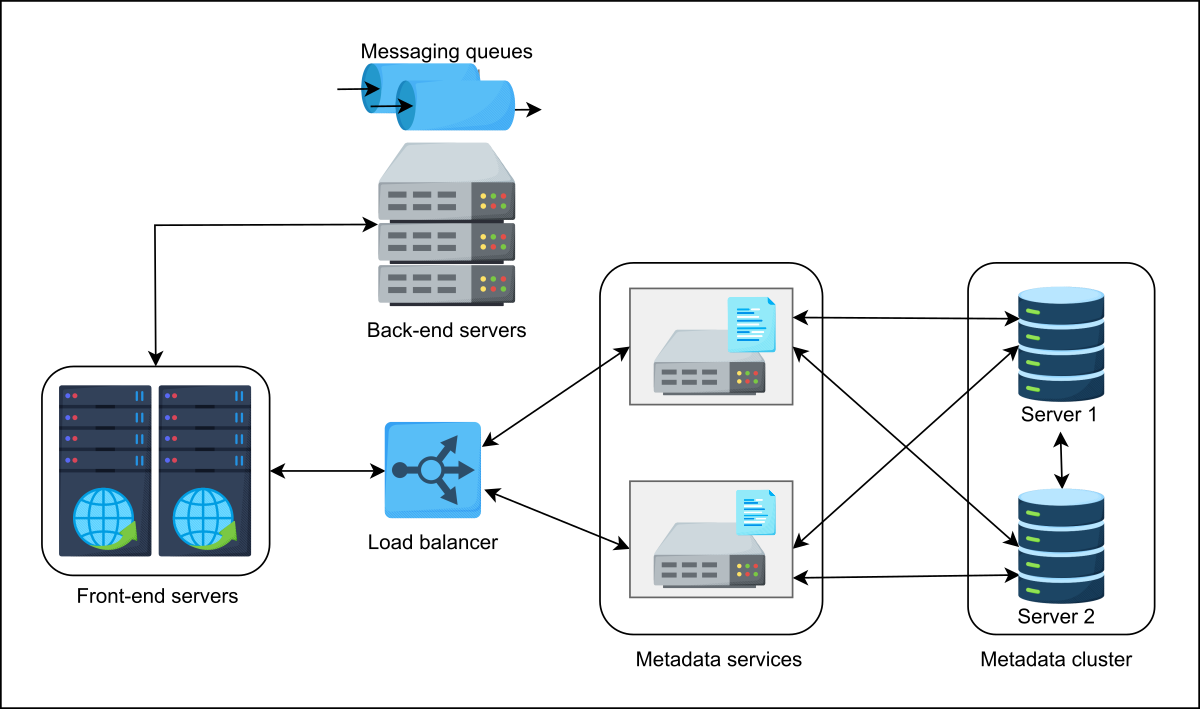
\includegraphics[width=0.5\textwidth]{Images/chapter_17/section_6330012742975488/5009934834335744.png}
 \caption{A load balancer is introduced between the front-end servers and metadata services}
\end{figure}

\begin{enumerate}
\setcounter{enumi}{1}
\item
\protect\phantomsection\label{1XU9rTaDGM-Bv_osM9tqA}
If the metadata that needs to be stored is too large, then one of the following modes can be followed:
\end{enumerate}

\begin{itemize}
\item
\protect\phantomsection\label{2L8-1UZJkSzSlQnCGuDp2}
The first strategy is to use the sharding approach to divide data into different shards. \textbf{Sharding} can be performed based on some partition key or hashing techniques, as was discussed in the lesson on \href{https://www.educative.io/courses/grokking-the-system-design-interview/data-partitioning}{database partitioning}. Each shard is stored on a different host in the cluster. Moreover, each shard is also replicated on different hosts to enhance availability. In this cluster-organization approach, the front-end server has a mapping table between shards and the hosts. Therefore, the front-end server is responsible for redirecting requests to the host where the data is stored.
\end{itemize}

\begin{figure}[htbp]
 \centering
 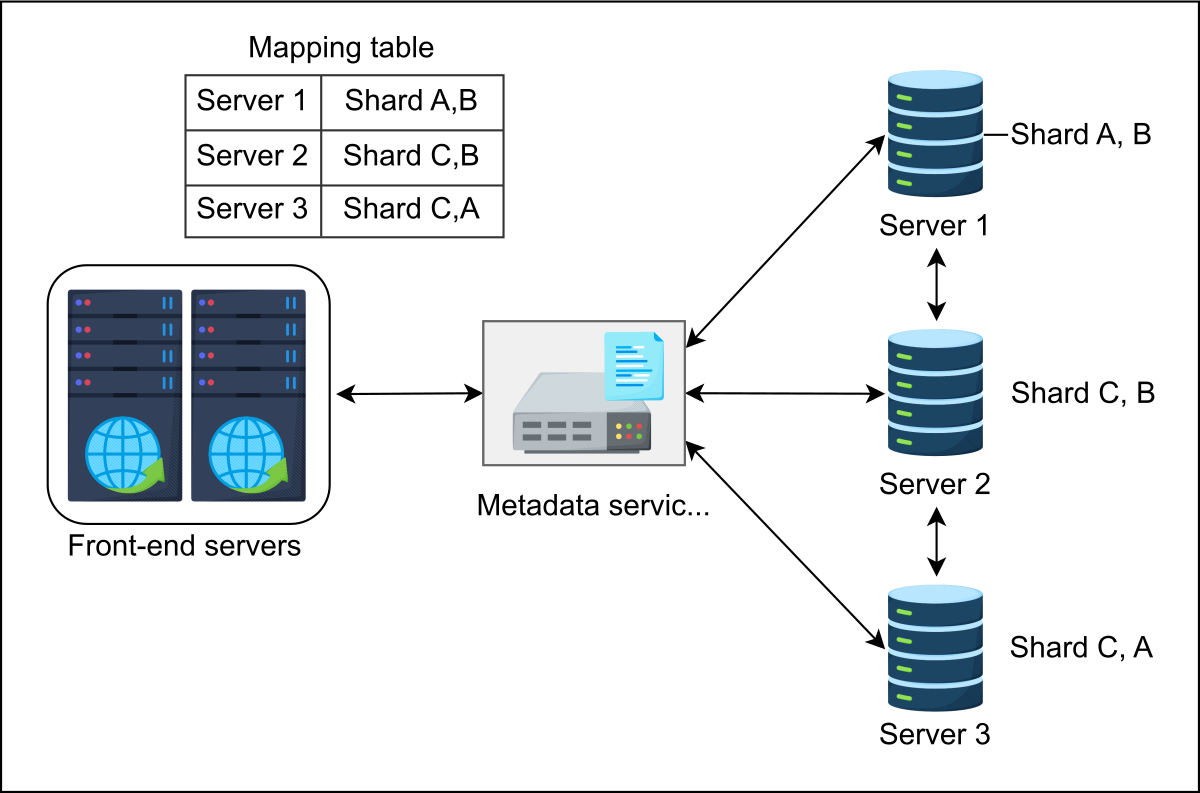
\includegraphics[width=0.5\textwidth]{Images/chapter_17/section_6330012742975488/6382605241286656.png}
 \caption{Mapping table resides on the front-end servers}
\end{figure}

\begin{itemize}
\item
\protect\phantomsection\label{VU6M7Fb5AFe9trR57xfll}
The second approach is similar to the first one. However, the mapping table in this approach is stored on each host instead of just on the front-end servers. Because of this, any random host can receive a request and forward it to the host where the data resides. This technique is suitable for read-intensive applications.
\end{itemize}

\begin{figure}[htbp]
 \centering
 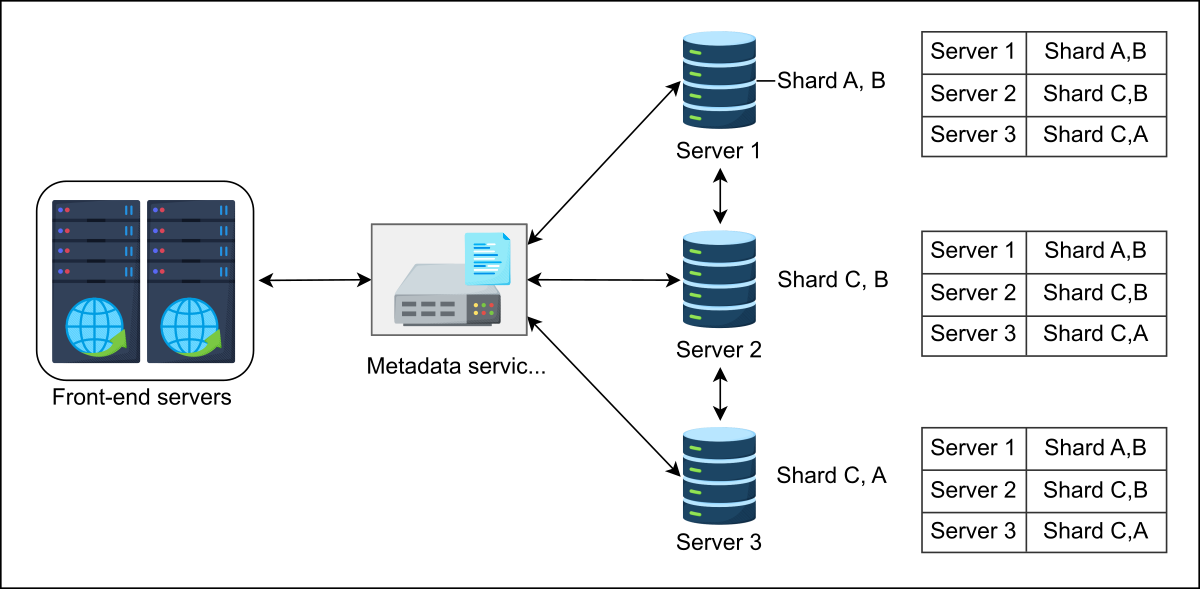
\includegraphics[width=0.5\textwidth]{Images/chapter_17/section_6330012742975488/5248957213442048.png}
 \caption{Mapping table resides on each metadata server}
\end{figure}

In our discussion on distributed messaging queues, we focused on the high-level design of this type of queue. Furthermore , we explored each component in the high-level design, including the following:

\begin{itemize}
\item
\protect\phantomsection\label{ofvNEeeeStEOGvaaI6_ni}
Front-end servers and the services required of them for smooth operations.
\item
\protect\phantomsection\label{sc8qIcncWFdl5DtJvrkcJ}
Load balancers.
\item
\protect\phantomsection\label{wZzLazt7gHC9z9wmFNToN}
Metadata services.
\item
\protect\phantomsection\label{t2meB6wsMddczM3R4i2tE}
Metadata clusters and their organization.
\end{itemize}
\\
A vital part of the design is the organization of servers at the back-end for queue creation, deletion, and other such operations. The next lesson focuses on the organization of back-end servers and the management of queues, along with other important operations related to message delivery and retrieval.

% End of section content